% 第 18 题四棱锥 P-ABCD：按固定源 PDF 的顶点相对位置重绘。
% 实线 5 条：PA、PB、PD、DA、AB；虚线 4 条：PC（棱锥的高）、CD、CB、CA。
% 虚线 CB 与实线 PA 在投影中相交（900 dpi 核对：PB 之外唯一交叉，实线压在上层）——先画虚线后画实线即得。
% E 为 AB 中点（实心圆点），与原题「E 为 AB 的中点」一致。
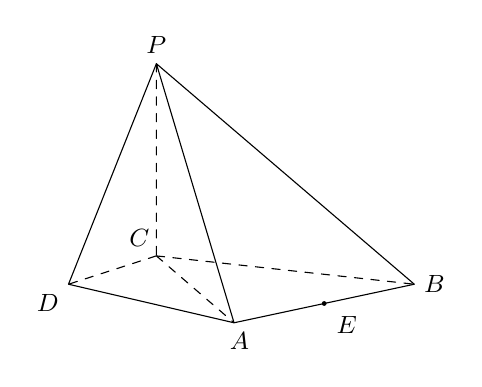
\begin{tikzpicture}[line cap=round,line join=round,font=\small,scale=0.72]
\coordinate (P) at (1.60,4.60);
\coordinate (C) at (1.60,1.21);
\coordinate (D) at (0.05,0.71);
\coordinate (B) at (6.15,0.71);
\coordinate (A) at (2.97,0.03);
\coordinate (E) at (4.56,0.37);
% 虚线先画（含 PC 竖线与底面后侧棱、对角线 CA）
\draw[dashed] (P)--(C) (C)--(D) (C)--(B) (C)--(A);
% 实线后画（压住虚线交叉处，与原图一致）
\draw (P)--(D) (P)--(B) (P)--(A) (D)--(A) (A)--(B);
\node[above] at (P) {$P$};
\node[above left,xshift=1pt] at (C) {$C$};
\node[below left] at (D) {$D$};
\node[right] at (B) {$B$};
\node[below,xshift=2pt] at (A) {$A$};
\fill (E) circle (1.2pt) node[below right,xshift=1pt,yshift=-1pt] {$E$};
\end{tikzpicture}
